%% Преамбула TeX-файла

% 1. Стиль и язык
\documentclass[utf8x, 14pt]{G7-32} % Стиль (по умолчанию будет 14pt)

% Остальные стандартные настройки убраны в preamble.inc.tex.
\sloppy

% Настройки стиля ГОСТ 7-32
% Для начала определяем, хотим мы или нет, чтобы рисунки и таблицы нумеровались в пределах раздела, или нам нужна сквозная нумерация.
\EqInChapter % формулы будут нумероваться в пределах раздела
\TableInChapter % таблицы будут нумероваться в пределах раздела
\PicInChapter % рисунки будут нумероваться в пределах раздела

% Добавляем гипертекстовое оглавление в PDF
\usepackage[
bookmarks=true, colorlinks=true, unicode=true,
urlcolor=black,linkcolor=black, anchorcolor=black,
citecolor=black, menucolor=black, filecolor=black,
]{hyperref}

\AfterHyperrefFix

\usepackage{microtype}% полезный пакет для микротипографии, увы под xelatex мало чего умеет, но под pdflatex хорошо улучшает читаемость

% Тире могут быть невидимы в Adobe Reader
\ifInvisibleDashes
\MakeDashesBold
\fi

% С такими оно полями оно работает по-умолчанию:
% \RequirePackage[left=20mm,right=10mm,top=20mm,bottom=20mm,headsep=0pt,includefoot]{geometry}
% Если вас тошнит от поля в 10мм --- увеличивайте до 20-ти, ну и про переплёт не забывайте:
\geometry{right=20mm}
\geometry{left=30mm}
\geometry{bottom=20mm}
\geometry{ignorefoot}% считать от нижней границы текста


% Пакет Tikz
\usepackage{tikz}
\usetikzlibrary{arrows,positioning,shadows}

% Произвольная нумерация списков.
\usepackage{enumerate}

% ячейки в несколько строчек
\usepackage{multirow}

% itemize внутри tabular
\usepackage{paralist,array}

%\setlength{\parskip}{1ex plus0.5ex minus0.5ex} % разрыв между абзацами
\setlength{\parskip}{1ex} % разрыв между абзацами
\usepackage{blindtext}

% Центрирование подписей к плавающим окружениям
%\usepackage[justification=centering]{caption}

\usepackage{newfloat}
\DeclareFloatingEnvironment[
placement={!ht},
name=Equation
]{eqndescNoIndent}
\edef\fixEqndesc{\noexpand\setlength{\noexpand\parindent}{\the\parindent}\noexpand\setlength{\noexpand\parskip}{\the\parskip}}
\newenvironment{eqndesc}[1][!ht]{%
    \begin{eqndescNoIndent}[#1]%
\fixEqndesc%
}
{\end{eqndescNoIndent}}

\usepackage{float}

\usepackage{pdfpages}

\usepackage{graphicx} % для вставки рисунков
\graphicspath{{image/}}
\DeclareGraphicsExtensions{.pdf, .png, .jpg}

\usepackage{wrapfig}

\newcommand{\rouble}{{\rm{P}\kern-.635em\rule[.5ex]{.52em}{.04em}\kern.11em}}

% Настройки листингов.
\ifPDFTeX
% 8 Листинги

\usepackage{listings}

% Значения по умолчанию
\lstset{
  basicstyle= \footnotesize,
  breakatwhitespace=true,% разрыв строк только на whitespacce
  breaklines=true,       % переносить длинные строки
%   captionpos=b,          % подписи снизу -- вроде не надо
  inputencoding=koi8-r,
  numbers=left,          % нумерация слева
  numberstyle=\footnotesize,
  showspaces=false,      % показывать пробелы подчеркиваниями -- идиотизм 70-х годов
  showstringspaces=false,
  showtabs=false,        % и табы тоже
  stepnumber=1,
  tabsize=4,              % кому нужны табы по 8 символов?
  frame=single
}

% Стиль для псевдокода: строчки обычно короткие, поэтому размер шрифта побольше
\lstdefinestyle{pseudocode}{
  basicstyle=\small,
  keywordstyle=\color{black}\bfseries\underbar,
  language=Pseudocode,
  numberstyle=\footnotesize,
  commentstyle=\footnotesize\it
}

% Стиль для обычного кода: маленький шрифт
\lstdefinestyle{realcode}{
  basicstyle=\scriptsize,
  numberstyle=\footnotesize
}

% Стиль для коротких кусков обычного кода: средний шрифт
\lstdefinestyle{simplecode}{
  basicstyle=\footnotesize,
  numberstyle=\footnotesize
}

% Стиль для BNF
\lstdefinestyle{grammar}{
  basicstyle=\footnotesize,
  numberstyle=\footnotesize,
  stringstyle=\bfseries\ttfamily,
  language=BNF
}

% Определим свой язык для написания псевдокодов на основе Python
\lstdefinelanguage[]{Pseudocode}[]{Python}{
  morekeywords={each,empty,wait,do},% ключевые слова добавлять сюда
  morecomment=[s]{\{}{\}},% комменты {а-ля Pascal} смотрятся нагляднее
  literate=% а сюда добавлять операторы, которые хотите отображать как мат. символы
    {->}{\ensuremath{$\rightarrow$}~}2%
    {<-}{\ensuremath{$\leftarrow$}~}2%
    {:=}{\ensuremath{$\leftarrow$}~}2%
    {<--}{\ensuremath{$\Longleftarrow$}~}2%
}[keywords,comments]

% Свой язык для задания грамматик в BNF
\lstdefinelanguage[]{BNF}[]{}{
  morekeywords={},
  morecomment=[s]{@}{@},
  morestring=[b]",%
  literate=%
    {->}{\ensuremath{$\rightarrow$}~}2%
    {*}{\ensuremath{$^*$}~}2%
    {+}{\ensuremath{$^+$}~}2%
    {|}{\ensuremath{$|$}~}2%
}[keywords,comments,strings]

% Подписи к листингам на русском языке.
\renewcommand\lstlistingname{Листинг}
\renewcommand\lstlistlistingname{Листинги}

\else
\usepackage{local-minted}
\fi

% Полезные макросы листингов.
% Любимые команды
\newcommand{\Code}[1]{\textbf{#1}}


% Стиль титульного листа и заголовки


\begin{document}
%% НАЧАЛО ТИТУЛЬНОГО ЛИСТА
\begin{center}

	\textit{
		\normalsize{Федеральное государственное бюджетное образовательное учреждение высшего профессионального образования
}}\\ 
	
	\textit{
		\normalsize  {\bf  «Московский государственный технический университет}\\ 
		\normalsize  {\bf имени Н. Э. Баумана»}\\
		\normalsize  {\bf (МГТУ им. Н.Э. Баумана)}\\
	}
	\noindent\rule{\textwidth}{2pt}
	\hfill \break
	\noindent
	\makebox[0pt][l]{ФАКУЛЬТЕТ}%
	\makebox[\textwidth][c]{«Информатика и системы управления»}%
	\\
	\noindent
	\makebox[0pt][l]{КАФЕДРА}%
	\makebox[\textwidth][c]{«Программное обеспечение ЭВМ}
	\\{ и информационные технологии»}%
	\\
	\hfill\break
	\hfill \break
	\hfill \break
	\hfill \break
	\normalsize{\bf РАСЧЁТНО - ПОЯСНИТЕЛЬНАЯ ЗАПИСКА}\\
	\normalsize{\bf к курсовому проекту на тему:}\\
	\hfill \break
	\large{Визуализация взаимодействия частиц при столкновении (взрыв)}\\
	\hfill \break
	\hfill \break
	\hfill \break
	\hfill \break
	\hfill \break	
	\normalsize {
		\noindent
		\makebox[0pt][l]{Студент}%
		\makebox[\textwidth][c]{}%
		\makebox[0pt][r]{{$\underset{\text{(Подпись, дата)}}{\underline{\hspace{6cm}}}$ \space Сиденко А. Г. }}
	}\\
	\hfill \break	
	\normalsize {
		\noindent
		\makebox[0pt][l]{Руководитель курсового проекта}%
		\makebox[\textwidth][c]{ ~~~~~~~~      }%
		\makebox[0pt][r]{{$\underset{\text{(Подпись, дата)}}{\underline{\hspace{4cm}}}$ \space Кострицкий А. С. }}
	}
\end{center}

\hfill

\begin{center} Москва 2019

\end{center}

\thispagestyle{empty} % 
% КОНЕЦ ТИТУЛЬНОГО ЛИСТА


\includepdf[pages=-]{image/rpz_titul.pdf}
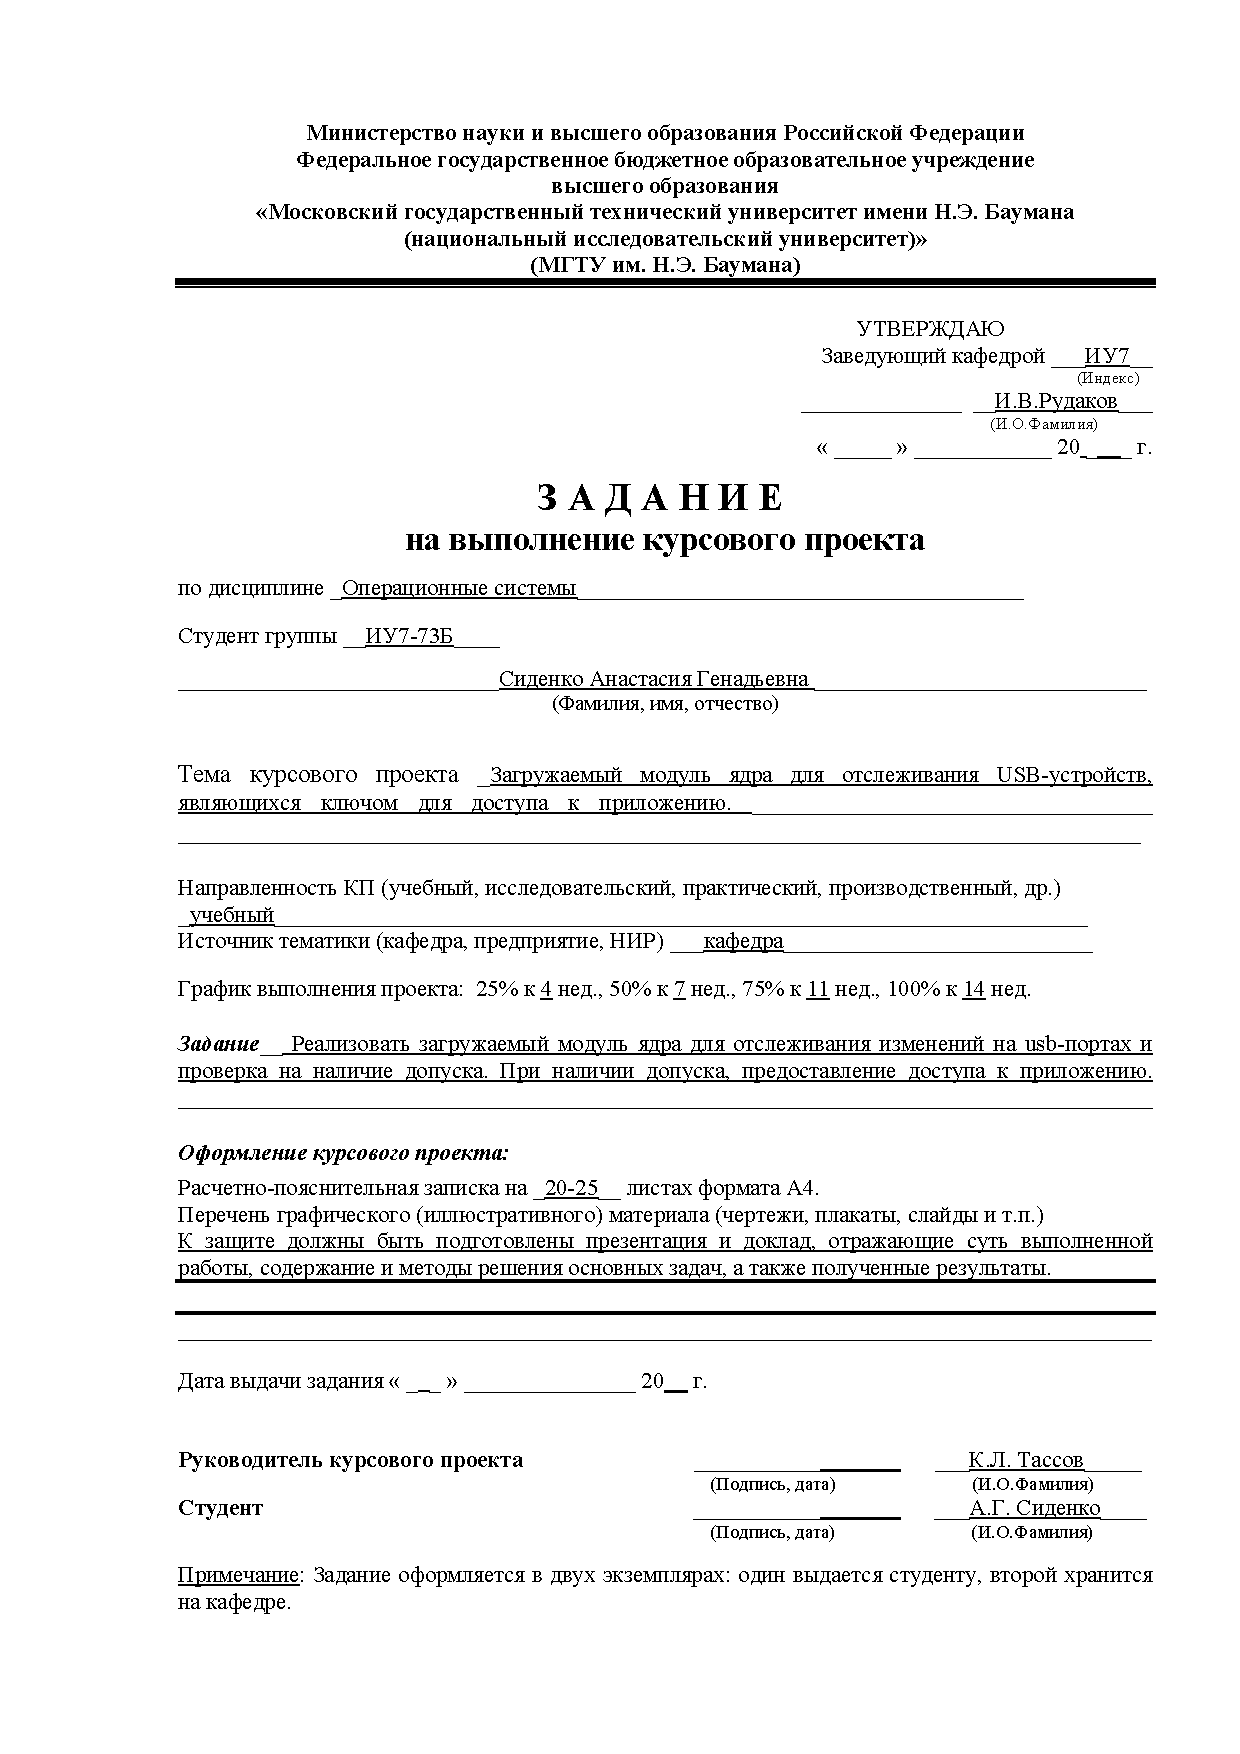
\includepdf[pages=-]{image/tz.pdf}

\frontmatter % выключает нумерацию ВСЕГО; здесь начинаются ненумерованные главы: реферат, введение, глоссарий, сокращения и прочее.

% Также можно использовать \Referat, как в оригинале
\Referat

\hfill

Курсовой проект представляет собой загружаемого модуля ядра для отслеживания USB-устройств, являющихся ключом для доступа к приложению.

Ключевые слова: загружаемый модуль, Linux, USB устройство, уведомитель(notify), шифрование. 

Отчёт содержит \pageref{LastPage}\,~страниц%
    \ifnum \totfig >0
    , \totfig~рисунка%
    \fi
    \ifnum \tottab >0
    , \tottab~таблицы%
    \fi
    %
    \ifnum \totbib >0
    , \totbib~источников%
    \fi
    %
    \ifnum \totapp >0
    , \totapp~прил.%
    \else
    .%
    \fi

%%% Local Variables: 
%%% mode: latex
%%% TeX-master: "rpz"
%%% End: 


\tableofcontents
%\printnomenclature % Автоматический список сокращений

\Introduction

\hfill

В настоящее время кража персональных данных -- это большая проблема во всем мире. Одним из способов защиты ваших персональных данных на компьютере, это доступ к ним по USB-устройству \cite{statcriminal}. 

Если вы не хотите, чтобы кто-то извлекал документы с Вашего компьютера через USB или устанавливал вредоносные программы, необходимо отслеживать USB-устройства, их идентифицировать и предоставлять или отказывать в доступе.

Linux -- это операционная система с монолитным ядром. Для того, чтобы избежать перекомпиляции ядра при добавлении нового функционала, используются загружаемые модули ядра.  Целью данной работы является реализация загружаемого модуля ядра для отслеживания USB-устройств, являющихся ключом для доступа к приложению.

Необходимая функциональность.
\begin{enumerate}
	\item[1. ]  Список разрешенных устройств.
	\item[2. ]  Список секретных файлов, приложений.
	\item[3. ]  Предоставление или отказ в доступе, при наличии различных USB-устройств.
\end{enumerate}
	
	Для достижения поставленной цели необходимо решить следующие задачи. 
	\begin{enumerate}
		\item[1. ] Определение основных понятий. 
		\item[2. ] Разработка алгоритмов. 
		\item[3. ] Реализация загружаемого модуля. 
	\end{enumerate}





\mainmatter % это включает нумерацию глав и секций в документе ниже

\chapter{\textbf{Аналитический раздел}}
\hfill

Целью данной работы является реализация загружаемого модуля ядра для отслеживания USB­-устройств, являющихся ключом для доступа к приложению. В данном разделе производится постановка задачи и рассмотрение основных понятий. 

\section{\textbf{Постановка задачи}}

Требуется разработать программное обеспечение для отслеживания USB­-устройств, который обладает следующей функциональностью:
\begin{itemize}
\item список разрешенных устройств;
\item список путей к секретным файлам;
\item отслеживание появления новых USB­-устройств;
\begin{itemize}
\item если устройство известно, происходит расшифровка файла;
\item если устройство не известно, происходит зашифровка файла. 
\end{itemize}
\end{itemize}

На вход подается USB устройство с паролем. На выходе получаем зашифрованный или расшифрованный файл.

\section{\textbf{Загружаемый модуль ядра}}

Ядро Linux динамически изменяемое -- это означает, что вы можете загружать в ядро дополнительную функциональность, выгружать функции из ядра и даже добавлять новые модули, использующие другие модули ядра. Преимущество загружаемых модулей заключается в возможности сократить расход памяти для ядра, загружая только необходимые модули (это может оказаться важным для встроенных систем).

Загружаемый модуль представляет собой специальный объектный файл в формате ELF (Executable and Linkable Format). Обычно объектные файлы обрабатываются компоновщиком, который разрешает символы и формирует исполняемый файл. Однако в связи с тем, что загружаемый модуль не может разрешить символы до загрузки в ядро, он остается ELF-объектом. Для работы с загружаемыми модулями можно использовать стандартные средства работы с объектными файлами (имеют суффикс .ko, от kernel object). \cite{kernelmodules}


В OC Linux существуют специальные команды для работы с загружаемыми модулями ядра.

insmod -- Загружает модуль в ядро из конкретного файла, если модуль зависит от других модулей. Только суперпользователь может загрузить модуль в ядро.

lsmod -- Выводит список модулей, загруженных в ядро.

modinfo -- Извлекает информацию из модулей ядра (лицензия, автор, описание и т.д.).

rmmod -- Команда используется для выгрузки модуля из ядра, в качестве параметра передается имя файла модуля. Только суперпользователь может выгрузить модуль из ядра.

Загружаемые модули ядра должны содержать два макроса module\_init и module\_exit.

\section{\textbf{Уведомления в ядре Linux}}

\subsection{\textbf{Уведомители}}

Ядро Linux содержит механизм, называемый <<уведомителями>> (notifiers) или <<цепочками уведомлений>> (notifiers chains), который позволяет различным подсистемам подписываться на асинхронные события от других подсистем. Цепочки уведомлений в настоящее время активно используется в ядре; существуют цепочки для событий hotplug памяти, изменения политики частоты процессора, события USB hotplug, загрузка и выгрузка модулей, перезагрузки системы, изменения сетевых устройств и т. д. \cite{notifications}

Основной является структура notifier\_block, листинг которой представлен в \ref{lst:notifier_block}.

 \begin{lstlisting}[caption = Структура notifier\_block, label =  lst:notifier_block]
 struct notifier_block {
    notifier_fn_t notifier_call;
    struct notifier_block __rcu *next;
    int priority;
 };
 \end{lstlisting}
 
Структура определен в \#include/linux/notifier.h. Эта структура содержит указатель на функцию обратного -- notifier\_call, ссылку на следующий notifier\_block и приоритет функции, функции с более высоким приоритетом выполняются первыми.

\subsection{\textbf{Уведомитель изменений на USB портах}}

Существует уведомитель, позволяющий отслеживать изменения на usb портах. \cite{usbnotifications}

\textit{void usb\_register\_notify(struct notifier\_block *nb);}

\textit{void usb\_unregister\_notify(struct notifier\_block *nb);}

Существующие события: \textit{USB\_DEVICE\_ADD} -- добавление нового устройства, \textit{USB\_DEVICE\_REMOVE} -- удаление устройства.

\section{\textbf{Хранение информации о доступных USB устройствах}}

Для хранения устройств будет использовать двусвязный список ядра Linux, реализованный в файле \#include/linux/list.h. \cite{lists}

\textit{LIST\_HEAD} -- объявление и инициализация головы списка.

\textit{list\_for\_each\_entry(temp, \&connected\_devices, list\_node)} -- проход по списку.

\textit{list\_for\_each\_entry\_safe(device, temp, \&connected\_devices, list\_node)} -- «защищенный» проход по всем элементам списка, используется для удаления записей списка.

\textit{list\_add\_tail(struct list\_head * new, struct list\_head * head) }-- добавление нового элемента.

\section{\textbf{Вызов приложений пользовательского пространства из ядра}}

Usermode-helper API -- это простой API с известным набором опций. Например, чтобы создать процесс из пользовательского пространства, обычно необходимо указать имя исполняемого файла, параметры исполняемого файла и набор переменных среды. \cite{userspace}

\textit{int call\_usermodehelper(const char *path, char **argv, char **envp, int wait)} -- подготовить и запустить приложение пользовательского режима.

\textit{const char * path} -- путь к исполняемому файлц пользовательского режима.

\textit{char ** argv} -- параметры.

\textit{char ** envp} --  переменные среды.

\textit{int wait}  -- дождитесь завершения работы приложения и возврата статуса.

Реализация usermodehelper проста и понятна, рисунок \ref{img:user_kernel}.

\textit{UMH\_WAIT\_PROC} -- если запрашивающий хочет дождаться завершения всего процесса, включая вызов пользовательского пространства, \textit{UMH\_NO\_WAIT} -- вообще не ждать, \textit{UMH\_WAIT\_EXEC} -- дождаться вызова приложения пользовательского пространства, но не завершения.

\begin{figure}[H]
	\centering
	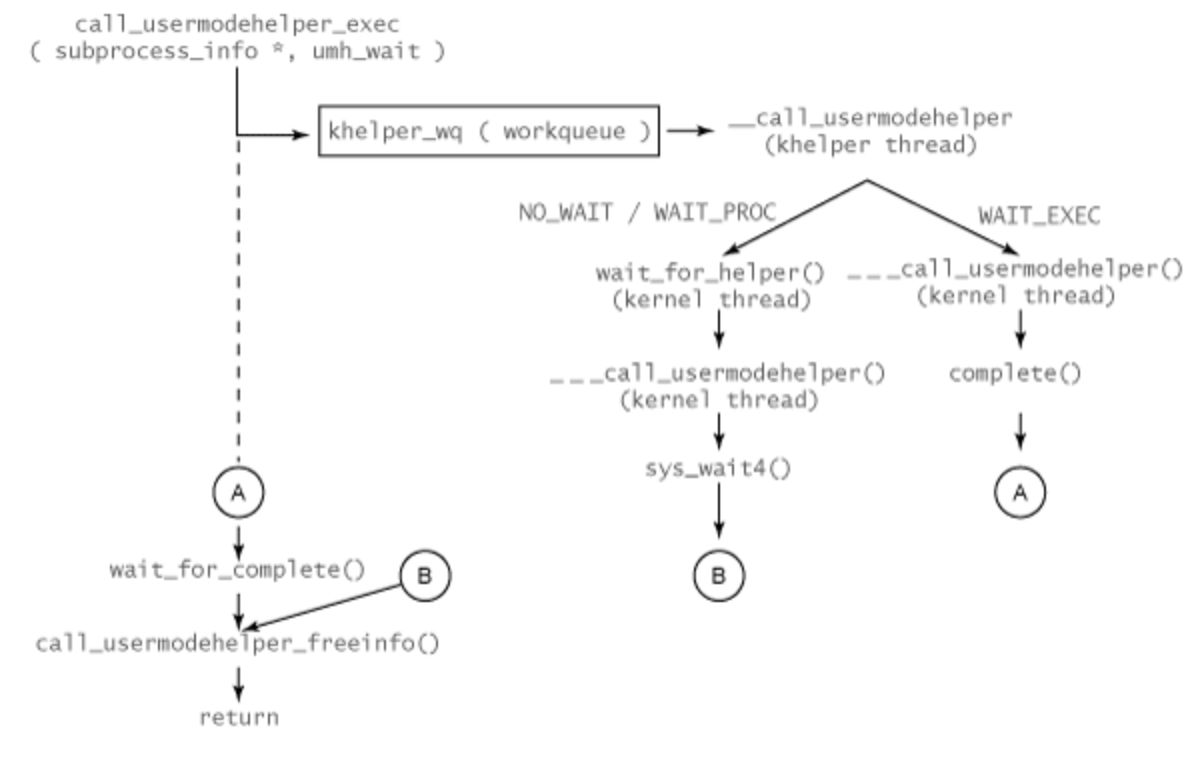
\includegraphics[scale=0.8]{user_kernel}
	\caption{Внутренняя реализация API usermodehelper. }
	\label{img:user_kernel}
\end{figure}

\section{\textbf{Чтение и запись файлов в пространстве ядра}}

Иногда необходимо читать и записывать файловые данные в ядре Linux. \cite{read_write}

В основном это функции: 

\textit{struсt file* filp\_open(const char* filename, int open\_mode, int mode)} -- открытие файла в ядре. filename -- имя файла, который может быть создан или открыт, включает путь до файла; open\_mode -- режим открытия файла O\_CREAT, O\_RDWR, O\_RDONLY, mode -- используется при создании файла, установите разрешения на чтение и запись созданного файла, в противном случае он может быть установлен в 0.

\textit{int filp\_close(struct file*filp, fl\_owner\_t id)} -- закрытие файла.
 
\textit{ssize\_t vfs\_read(struct file* filp, char \_\_user* buffer, size\_t len, loff\_t* pos)}, \textit{ssize\_t vfs\_write(struct file* filp, const char \_\_user* buffer, size\_t len, loff\_t* pos)} -- чтение и запись файлов в ядре.

Второй параметр этих двух функций имеет перед собой модификатор \_\_user, который требует, чтобы оба указателя буфера указывали на память пространства пользователя. Чтобы эти две функции чтения и записи правильно работали с указателем буфера в пространстве ядра, вам нужно использовать функцию set\_fs(). Ее функция состоит в том, чтобы изменить способ, которым ядро обрабатывает проверку адресов памяти. На самом деле параметр fs этой функции имеет только два значения: USER\_DS и KERNEL\_DS, которые представляют пространство пользователя и пространство ядра соответственно.

\textit{void set\_fs(mm\_segment\_t fs)}

\textit{mm\_segment\_t  get\_fs ()}

\section{\textbf{Основные используемые структуры}}

В данной работе происходит отслеживание изменений на usb портах, основными структурами являются usb\_device и usb\_device\_id.

\subsection{\textbf{usb\_device}}

Структура usb\_device приведена в листинге \ref{lst:usb_device} -- представление USB-устройста в ядре.

Используемые поля:

descriptor -- дескриптор USB устройства. 

Каждое продающееся устройство с USB требует сертификации на соответствие требованиям USB, для чего ему необходимо иметь ID поставщика (vendor ID) и ID изделия (product ID). Эти поля присутствуют в descriptor, используются для идентификации USB устройства. 

\subsection{\textbf{usb\_device\_id}}

Структура usb\_device\_id приведена в листинге \ref{lst:usb_device_id} -- идентификация USB устройств для отслеживания и подключения.

Используемые поля:

idVendor -- ID поставщика; 

idProduct -- ID изделия.

\section{\textbf{Вывод}}

В данном разделе была постановлена задача и рассмотрены основные понятия. 
\chapter{\textbf{Конструкторский раздел}}

\hfill

Разрабатываемое программное обеспечения можно разделить на подзадачи:
\begin{itemize}
\item загружаемый модуль ядра;
\item приложение для шифрования файлов.
\end{itemize}

\section{\textbf{Перехват сообщений}}

\hfill

Для перехвата сообщений добавление нового USB устройства и удаление USB устройства необходимо в загружаемом модуле ядра разместить уведомитель, принимающий в качества параметра функцию обратного вызова нашей обработки данного события.

Для этого была создана следующая структура представленная в листинге \ref{lst:usb_notify}.

 \begin{lstlisting}[caption = Структура usb\_notify, label =  lst:usb_notify]
static struct notifier_block usb_notify = {
    .notifier_call = notify,
};
 \end{lstlisting}
 
 В этой структуре содержится указатель на прототип нашей функции обработки:

\textit{static int notify(struct notifier\_block *self, unsigned long action, void *dev)}

Для создания уведомителя передаем созданную структуру в функцию:

\textit{usb\_register\_notify(\&usb\_notify);}

Для удаления уведомителя передаем структуру в функцию:

\textit{usb\_unregister\_notify(\&usb\_notify);}

\section{\textbf{Хранение информации}}

\hfill

Для хранения информации о подключенных USB устройствах создадим структуру, листинг \ref{lst:our_usb_device}.

 \begin{lstlisting}[caption = Структура our\_usb\_device, label =  lst:our_usb_device]
typedef struct our_usb_device {
    struct usb_device_id dev_id;
    struct list_head list_node;
} our_usb_device_t;
 \end{lstlisting}
 
 Инициализируем список: \textit{LIST\_HEAD(connected\_devices);}

Для добавления нового подключенного устройства используется функция \ref{lst:add_usb},  для удаления -- \ref{lst:del_usb}.

\section{\textbf{Алгоритм работы функции-обработчика}}

На рисунке \ref{img:alg} представлен алгоритм работы функции обратного вызова добавления или удаления USB устройства.

\begin{figure}[H]
	\centering
	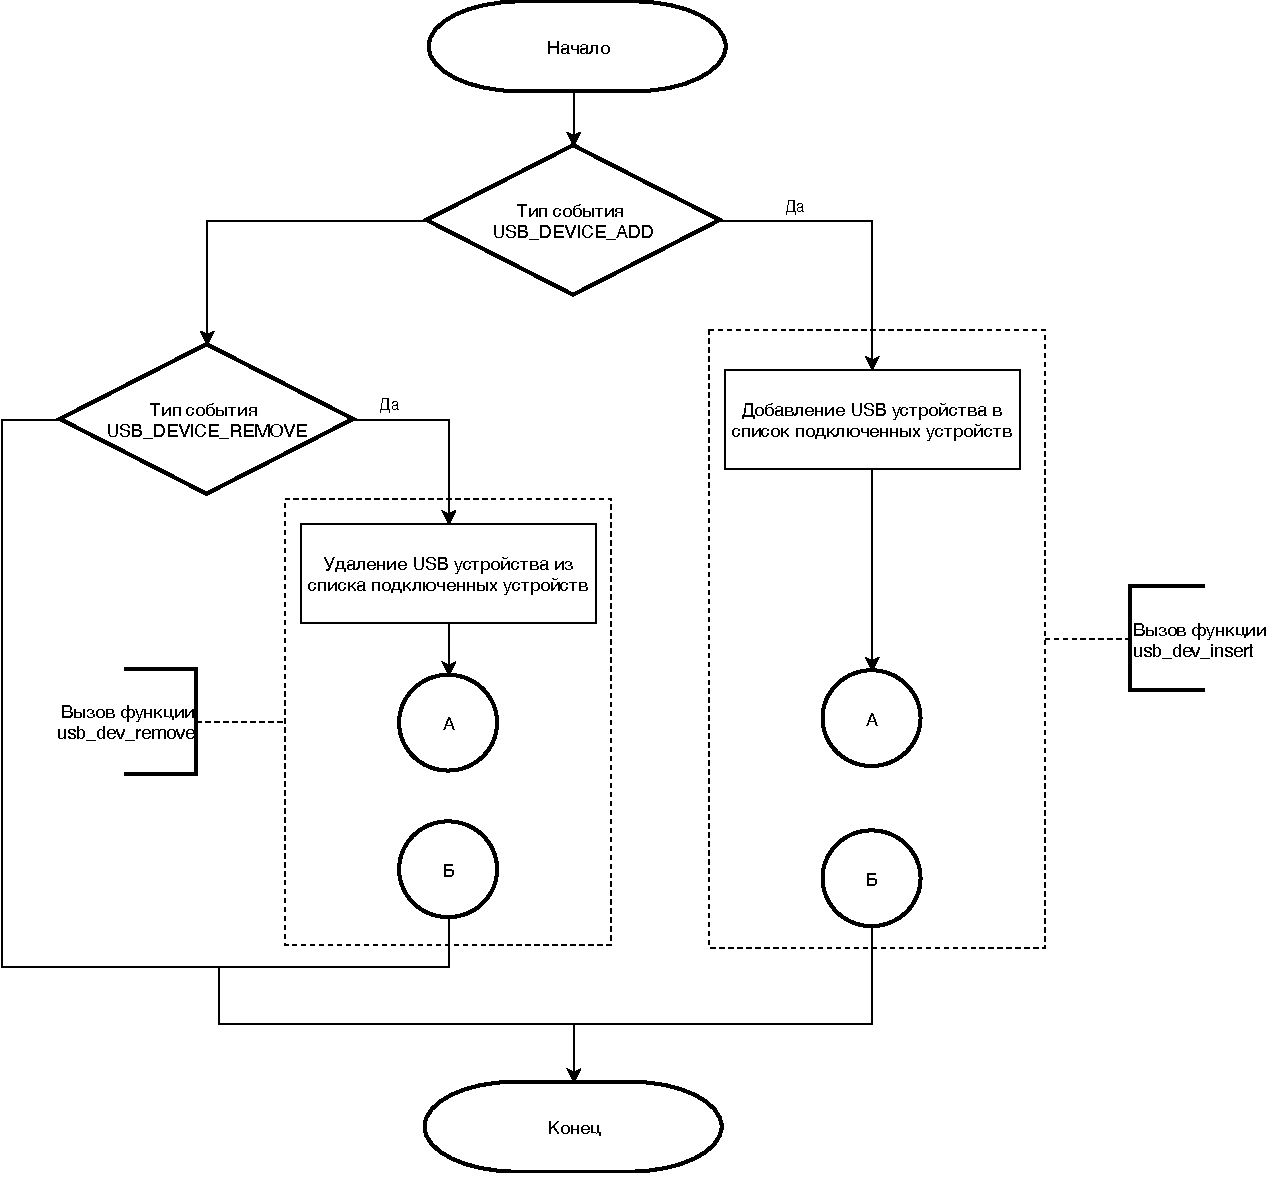
\includegraphics[scale=0.8]{alg1}
	\caption{Алгоритм работы функции-обработчика. }
	\label{img:alg}
\end{figure}

\begin{figure}[H]
	\centering
	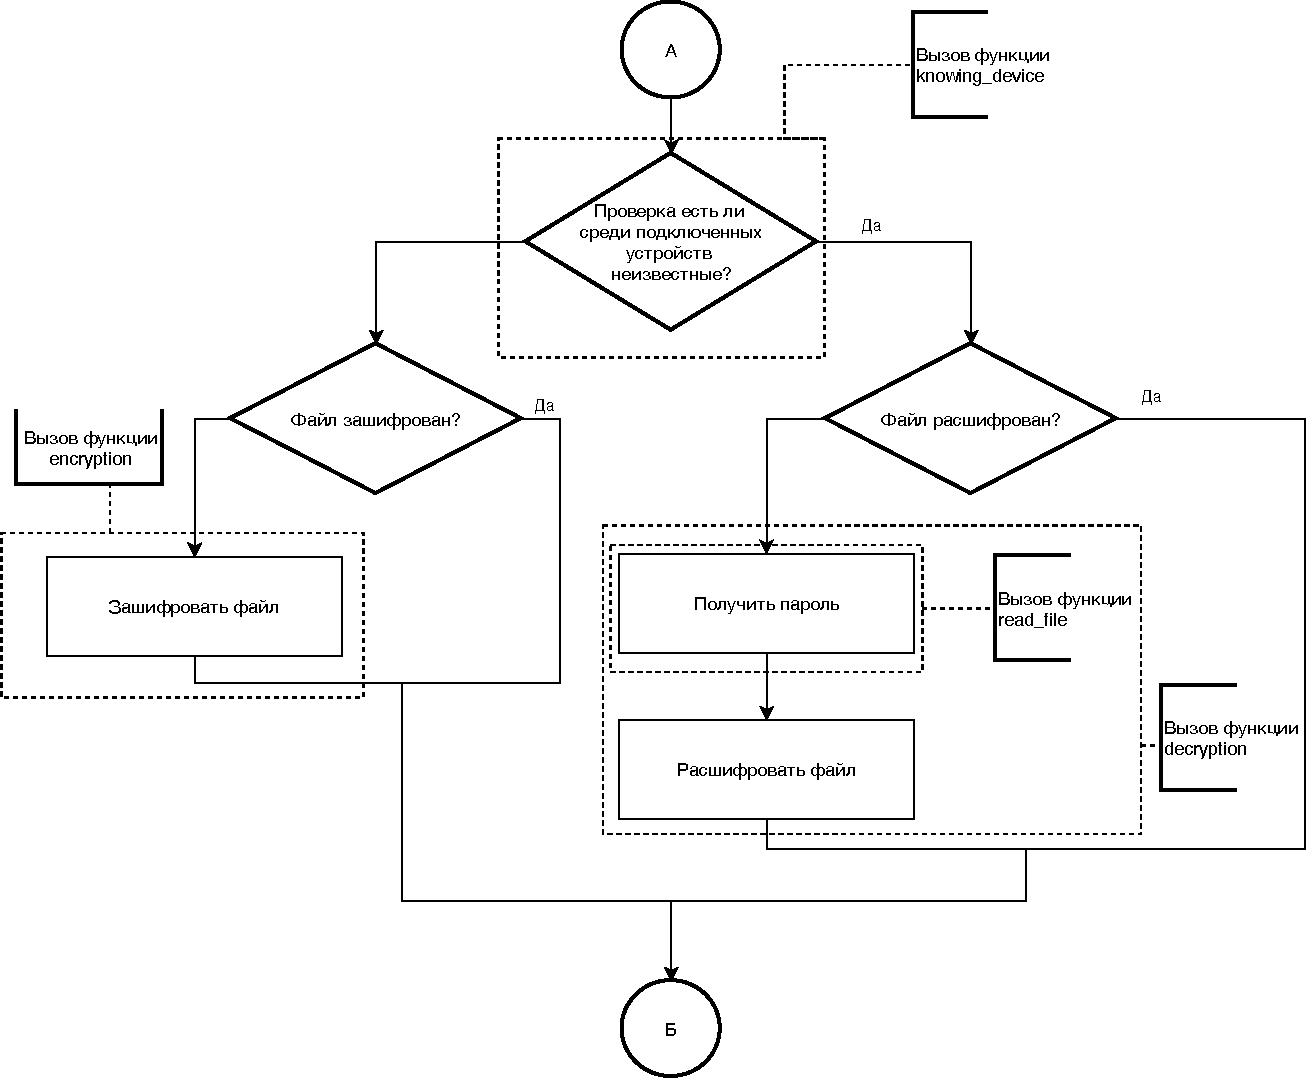
\includegraphics[scale=0.8]{alg2}
	\caption{Алгоритм работы функции-обработчика. }
	\label{img:alg1}
\end{figure}

\section{\textbf{Алгоритм шифрования файла}}

Для каждого файла из списка секретных.
 
\begin{enumerate}
\item[1. ] Побайтовое считывание символов из файла. 
\item[2. ] Применение операции XOR для данных с паролем. 
\item[3. ] Побайтовая запись символов в файл.  
\end{enumerate}


\section{\textbf{Вывод}}

\hfill

Структура программного обеспечения разработана, переход к реализации. 

\chapter{\textbf{Технологический раздел}}

\hfill

В соответствии с выбранной задачей -- реализация загружаемого модуля ядра для отслеживания USB-устройств, являющихся ключом для доступа к приложению. Необходимо выбрать средства реализации, создать модули и интерфейс, описать ограничения и порядок работы программы. 

\section{\textbf{Выбор технологий}}

Для реализации был выбран язык программирования C. Компилятор -- gcc. Для облегчения сборки был написан Makefile, позволяющий запускать сборку одной командой, листинг \ref{lst:makefile}.

\section{\textbf{Хранение данных }}

Параметры USB устройств, идентификатор поставщика и изделия, а также список секретных файлов и приложений хранятся в конфигурационном файле. Пример конфигурационного файла USB устройств представлен в листинге \ref{lst:config_usb}. Конфигурационный файл секретных файлов и приложений -- листинг \ref{lst:config_file}.

Пароль для доступа к зашифрованным данным хранится на разрешенном USB устройстве в файле \textit{password.txt}.

\section{\textbf{Загружаемый модуль}}

Цель работы создание загружаемого модуля, реализация загрузки и удаления представлена в листинге \ref{lst:module}.

После компиляции загружаемого модуля объектный файл может быть загружен в ядро с помощью команды \textit{insmod} с правами суперпользователя, для выгрузки используется команда \textit{rmmod}.

\section{\textbf{Функция-обработчик}}

В листинге \ref{lst:notify} представлена реализация функции обратного вызова добавления или удаления USB устройства \textit{static int notify(struct notifier\_block *self, unsigned long action, void *dev)}. 

С последующим вызовом, в зависимости от события \textit{static void usb\_dev\_remove(struct usb\_device *dev)}, \textit{static void usb\_dev\_insert(struct usb\_device *dev)}.

\section{\textbf{Проверка принадлежности устройства известным }}

Чтобы узнать можно ли расшифровать файл, необходимо узнать принадлежит ли устройство списку разрешенных устройств. Каждое устройство имеет уникальную пару идентификатор поставщика и идентификатор изделия, по ней и будет происходит поиск. Также в известных устройствах хранится файл с паролем для расшифровки секретных данных.

Реализация данной проверки представлена в листинге \ref{lst:check}.

Считывание пароля представлено в листинге \ref{lst:password}.

\section{\textbf{Проверка принадлежности устройства известным }}

После проверки принадлежности, при необходимости вызываются функции шифровки и расшифровки файлов, которые вызывают исполняемый файл пользовательского пространства.

Реализация этих функций представлена в листинге \ref{lst:user_call}.

\section{\textbf{Пример вывода в dmesg }}

На рисунке представлен пример работы загружаемого модуля.

\begin{figure}[H]
	\centering
	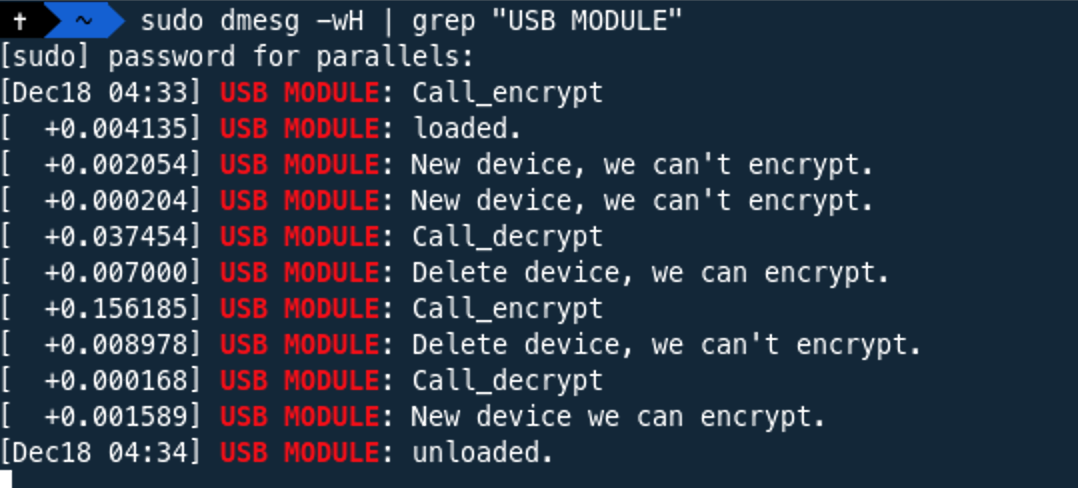
\includegraphics[scale=0.8]{example}
	\caption{Пример работы загружаемого модуля. }
	\label{img:example}
\end{figure}

\section{\textbf{Вывод}}

Реализовано спроектированное ПО, представлены результаты. 


\backmatter %% Здесь заканчивается нумерованная часть документа и начинаются ссылки и
            
\Conclusion % заключение к отчёту

\hfill

В результате проделанной работы выполнены следующие задачи.
\begin{enumerate}
		\item[1. ] Определены основные понятия, такие как загружаемый модуль ядра, уведомления и уведомители. Рассмотрены структуры usb\_device, usb\_device\_id. 
		\item[2. ] Разработаны алгоритмы работы функции-обработчика и шифрования файлов. 
		\item[3. ] Реализован загружаемого модуля. 
	\end{enumerate}
	
Достигнута цель проекта -- реализация загружаемого модуля ядра для отслеживания USB-устройств, являющихся ключом для доступа к приложению. 
%% заключение


% % Список литературы при помощи BibTeX
% Юзать так:
%
% pdflatex rpz
% bibtex rpz
% pdflatex rpz

\bibliographystyle{ugost2008}
\bibliography{rpz}
\nocite{*}
%%% Local Variables: 
%%% mode: latex
%%% TeX-master: "rpz"
%%% End: 


\appendix   % Тут идут приложения

\chapter{Листинги}

 \begin{lstlisting}[caption = Структура usb\_device, label =  lst:usb_device]
struct usb_device {
	int		devnum;
	char		devpath[16];
	u32		route;
	enum usb_device_state	state;
	enum usb_device_speed	speed;
	unsigned int		rx_lanes;
	unsigned int		tx_lanes;

	struct usb_tt	*tt;
	int		ttport;

	unsigned int toggle[2];

	struct usb_device *parent;
	struct usb_bus *bus;
	struct usb_host_endpoint ep0;

	struct device dev;

	struct usb_device_descriptor descriptor;
	struct usb_host_bos *bos;
	struct usb_host_config *config;

	struct usb_host_config *actconfig;
	struct usb_host_endpoint *ep_in[16];
	struct usb_host_endpoint *ep_out[16];

	char **rawdescriptors;

	unsigned short bus_mA;
	u8 portnum;
	u8 level;
	u8 devaddr;

	unsigned can_submit:1;
	unsigned persist_enabled:1;
	unsigned have_langid:1;
	unsigned authorized:1;
	unsigned authenticated:1;
	unsigned wusb:1;
	unsigned lpm_capable:1;
	unsigned usb2_hw_lpm_capable:1;
	unsigned usb2_hw_lpm_besl_capable:1;
	unsigned usb2_hw_lpm_enabled:1;
	unsigned usb2_hw_lpm_allowed:1;
	unsigned usb3_lpm_u1_enabled:1;
	unsigned usb3_lpm_u2_enabled:1;
	int string_langid;

	/* static strings from the device */
	char *product;
	char *manufacturer;
	char *serial;

	struct list_head filelist;

	int maxchild;

	u32 quirks;
	atomic_t urbnum;

	unsigned long active_duration;

#ifdef CONFIG_PM
	unsigned long connect_time;

	unsigned do_remote_wakeup:1;
	unsigned reset_resume:1;
	unsigned port_is_suspended:1;
#endif
	struct wusb_dev *wusb_dev;
	int slot_id;
	enum usb_device_removable removable;
	struct usb2_lpm_parameters l1_params;
	struct usb3_lpm_parameters u1_params;
	struct usb3_lpm_parameters u2_params;
	unsigned lpm_disable_count;

	u16 hub_delay;
	unsigned use_generic_driver:1;
};
 \end{lstlisting}
 
  \begin{lstlisting}[caption = Структура usb\_device\_id, label =  lst:usb_device_id]
 struct usb_device_id {
	/* which fields to match against? */
	__u16		match_flags;

	/* Used for product specific matches; range is inclusive */
	__u16		idVendor;
	__u16		idProduct;
	__u16		bcdDevice_lo;
	__u16		bcdDevice_hi;

	/* Used for device class matches */
	__u8		bDeviceClass;
	__u8		bDeviceSubClass;
	__u8		bDeviceProtocol;

	/* Used for interface class matches */
	__u8		bInterfaceClass;
	__u8		bInterfaceSubClass;
	__u8		bInterfaceProtocol;

	/* Used for vendor-specific interface matches */
	__u8		bInterfaceNumber;

	/* not matched against */
	kernel_ulong_t	driver_info
		__attribute__((aligned(sizeof(kernel_ulong_t))));
};
 \end{lstlisting}

  \begin{lstlisting}[caption = Добавление usb устройства, label =  lst:add_usb]
static void add_our_usb_device(struct usb_device *dev)
{
    our_usb_device_t* new_usb_device = (our_usb_device_t *)kmalloc(sizeof(our_usb_device_t), GFP_KERNEL);
    struct usb_device_id new_id = { USB_DEVICE(dev->descriptor.idVendor, dev->descriptor.idProduct) };
    new_usb_device->dev_id = new_id;
    list_add_tail(&new_usb_device->list_node, &connected_devices);
}
 \end{lstlisting}
 
  \begin{lstlisting}[caption = Удаление usb устройства, label =  lst:del_usb]
static void delete_our_usb_device(struct usb_device *dev)
{
    our_usb_device_t *device, *temp;
    list_for_each_entry_safe(device, temp, &connected_devices, list_node) 
    {
        if (device_match_device_id(dev, &device->dev_id))
        {
            list_del(&device->list_node);
            kfree(device);
        }
    }
}
 \end{lstlisting}
 
  \begin{lstlisting}[caption = Makefile, label =  lst:makefile]
ifneq ($(KERNELRELEASE),)
	obj-m := md.o
else
	CURRENT = $(shell uname -r)
	KDIR = /lib/modules/$(CURRENT)/build
	PWD = $(shell pwd)

default:
	$(MAKE) -C $(KDIR) M=$(PWD) modules

clean:
	rm -rf .tmp_versions
	rm *.ko
	rm *.o
	rm *.mod.c
	rm *.symvers
	rm *.order

endif
 \end{lstlisting}
 
   \begin{lstlisting}[caption = Конфигурационный файл USB устройств, label =  lst:config_usb]
 struct known_usb_device {
    struct usb_device_id dev_id;
    char *name;
};

// List of all USB devices you know
static const struct known_usb_device known_devices[] = {
    { .dev_id = { USB_DEVICE(0x058f, 0x6387) }, .name = "SAG" },
};
  \end{lstlisting}

   \begin{lstlisting}[caption = Конфигурационный файл секретных файлов и приложений, label =  lst:config_file]  
  static char *secret_apps[] = {
    "/home/parallels/Desktop/Operating_systems_coursework/file.txt",
    "/home/parallels/Desktop/Operating_systems_coursework/xor",
    "/usr/bin/firefox",
	NULL,
};
    \end{lstlisting}
 
   \begin{lstlisting}[caption = Загрузка и удаление модуля ядра, label =  lst:module]
static int __init my_module_init(void)
{
    usb_register_notify(&usb_notify);
    call_encryption();
    printk(KERN_INFO "USB MODULE: loaded.\n");
    return 0;
}

static void __exit my_module_exit(void)
{
    usb_unregister_notify(&usb_notify);    
    printk(KERN_INFO "USB MODULE: unloaded.\n");
}

module_init(my_module_init);
module_exit(my_module_exit);
 \end{lstlisting}
 
 
    \begin{lstlisting}[caption = Функция-обработчик, label =  lst:notify]
// If usb device inserted.
static void usb_dev_insert(struct usb_device *dev)
{   
    add_our_usb_device(dev);
    char *name = knowing_device();
    
    if (name)
    {
        if (state_encrypt)
            call_decryption(name);
        state_encrypt = false;
        printk(KERN_INFO "USB MODULE: New device we can encrypt.\n");
    }
    else
   {
        if (!state_encrypt)
            call_encryption();
        state_encrypt = true;
        printk(KERN_INFO "USB MODULE: New device, we can't encrypt.\n");
    }
}

// If usb device removed.
static void usb_dev_remove(struct usb_device *dev)
{
    delete_our_usb_device(dev);
    char *name = knowing_device();

    if (name)
    {
        if (state_encrypt)
            call_decryption(name);
        state_encrypt = false; 
        printk(KERN_INFO "USB MODULE: Delete device, we can encrypt.\n");
    }
    else
    {
        if (!state_encrypt)
            call_encryption();
        state_encrypt = true;
        printk(KERN_INFO "USB MODULE: Delete device, we can't encrypt.\n");
    }
}

// New notify.
static int notify(struct notifier_block *self, unsigned long action, void *dev)
{
    // Events, which our notifier react.
    switch (action) 
    {
        case USB_DEVICE_ADD:
            usb_dev_insert(dev);
	        break;
        case USB_DEVICE_REMOVE:
            usb_dev_remove(dev);
	        break;
        default:
	        break;
    }
    return 0;
}
 \end{lstlisting}
 
\begin{lstlisting}[caption = Функции для проверки разрешенных устройств, label =  lst:check]
// Match device id with device id.
static bool device_id_match_device_id(struct usb_device_id *new_dev_id, const struct usb_device_id *dev_id)
{
    // Check idVendor and idProduct, which are used.
    if (dev_id->idVendor != new_dev_id->idVendor)
        return false;
    if (dev_id->idProduct != new_dev_id->idProduct)
        return false;
    return true;
}

// Check our list of devices, if we know device.
static char *usb_device_id_is_known(struct usb_device_id *dev)
{
    unsigned long known_devices_len = sizeof(known_devices) / sizeof(known_devices[0]);
    int i = 0;
    for (i = 0; i < known_devices_len; i++)
    {
        if (device_id_match_device_id(dev, &known_devices[i].dev_id))
        {
            int size = sizeof(known_devices[i].name);
            char *name = (char *)kmalloc(size + 1, GFP_KERNEL);
            int j = 0;
            for (j = 0; j < size; j++)
                name[j] = known_devices[i].name[j];
            name[size + 1] = '\0';

            return name;
        }
    }
    return NULL;
}

static char *knowing_device(void)
{
    our_usb_device_t *temp;
    int count = 0;
    char *name;

    list_for_each_entry(temp, &connected_devices, list_node) {
        name = usb_device_id_is_known(&temp->dev_id);
        if (!name)
            return NULL;
        count++;
    }
    if (0 == count)
        return NULL;
    return name;
}
 \end{lstlisting}
 
 
    \begin{lstlisting}[caption = Считывание пароля из файла USB устройства, label =  lst:password]
static char *read_file(char *filename)
{
    struct kstat *stat;
    struct file *fp;
    mm_segment_t fs;
    loff_t pos = 0;
    char *buf;
    int size;

    fp = filp_open(filename, O_RDWR, 0644);
    if (IS_ERR(fp))
    {
        return NULL;
    }

    fs = get_fs();
    set_fs(KERNEL_DS);
    
    stat = (struct kstat *)kmalloc(sizeof(struct kstat), GFP_KERNEL);
    if (!stat)
    {
        return NULL;
    }

    vfs_stat(filename, stat);
    size = stat->size;

    buf = kmalloc(size, GFP_KERNEL);
    if (!buf) 
    {
        kfree(stat);
        return NULL;
    }

    kernel_read(fp, buf, size, &pos);

    filp_close(fp, NULL);
    set_fs(fs);
    kfree(stat);
    buf[size]='\0';
    return buf;
}
 \end{lstlisting}
 
 \begin{lstlisting}[caption = Функции вызывающие исполняемый файл пользовательского пространства, label =  lst:user_call]
 static int call_decryption(char *name_device) {
	printk(KERN_INFO "USB MODULE: Call_decrypt\n");
    
    char path[80];
    strcpy(path, USB_FOLDER);
    strcat(path, name_device);
    strcat(path, "/");
    strcat(path, PASSWORD_FILE);
    char *data = read_file(path);
	
    char *argv[] = {
     "/home/parallels/Desktop/Operating_systems_coursework/crypto",
    data,
    NULL };

    static char *envp[] = {
    "HOME=/",
    "TERM=linux",
    "PATH=/sbin:/bin:/usr/sbin:/usr/bin", 
     NULL };

    if (call_usermodehelper(argv[0], argv, envp, UMH_WAIT_PROC) < 0) 
    {
        return -1;
    }

    return 0;
}

static int call_encryption(void) {
    printk(KERN_INFO "USB MODULE: Call_encrypt\n");
    char *argv[] = {
     "/home/parallels/Desktop/Operating_systems_coursework/crypto",
    NULL };

    static char *envp[] = {
    "HOME=/",
    "TERM=linux",
    "PATH=/sbin:/bin:/usr/sbin:/usr/bin", 
    NULL };

    if (call_usermodehelper(argv[0], argv, envp, UMH_WAIT_PROC) < 0) 
    {
        return -1;
    }

    return 0;
}
  \end{lstlisting}
%%% Local Variables: 
%%% mode: latex
%%% TeX-master: "rpz"
%%% End: 


%\chapter{Листинги}

 \begin{lstlisting}[caption = Структура usb\_device, label =  lst:usb_device]
struct usb_device {
	int		devnum;
	char		devpath[16];
	u32		route;
	enum usb_device_state	state;
	enum usb_device_speed	speed;
	unsigned int		rx_lanes;
	unsigned int		tx_lanes;

	struct usb_tt	*tt;
	int		ttport;

	unsigned int toggle[2];

	struct usb_device *parent;
	struct usb_bus *bus;
	struct usb_host_endpoint ep0;

	struct device dev;

	struct usb_device_descriptor descriptor;
	struct usb_host_bos *bos;
	struct usb_host_config *config;

	struct usb_host_config *actconfig;
	struct usb_host_endpoint *ep_in[16];
	struct usb_host_endpoint *ep_out[16];

	char **rawdescriptors;

	unsigned short bus_mA;
	u8 portnum;
	u8 level;
	u8 devaddr;

	unsigned can_submit:1;
	unsigned persist_enabled:1;
	unsigned have_langid:1;
	unsigned authorized:1;
	unsigned authenticated:1;
	unsigned wusb:1;
	unsigned lpm_capable:1;
	unsigned usb2_hw_lpm_capable:1;
	unsigned usb2_hw_lpm_besl_capable:1;
	unsigned usb2_hw_lpm_enabled:1;
	unsigned usb2_hw_lpm_allowed:1;
	unsigned usb3_lpm_u1_enabled:1;
	unsigned usb3_lpm_u2_enabled:1;
	int string_langid;

	/* static strings from the device */
	char *product;
	char *manufacturer;
	char *serial;

	struct list_head filelist;

	int maxchild;

	u32 quirks;
	atomic_t urbnum;

	unsigned long active_duration;

#ifdef CONFIG_PM
	unsigned long connect_time;

	unsigned do_remote_wakeup:1;
	unsigned reset_resume:1;
	unsigned port_is_suspended:1;
#endif
	struct wusb_dev *wusb_dev;
	int slot_id;
	enum usb_device_removable removable;
	struct usb2_lpm_parameters l1_params;
	struct usb3_lpm_parameters u1_params;
	struct usb3_lpm_parameters u2_params;
	unsigned lpm_disable_count;

	u16 hub_delay;
	unsigned use_generic_driver:1;
};
 \end{lstlisting}
 
  \begin{lstlisting}[caption = Структура usb\_device\_id, label =  lst:usb_device_id]
 struct usb_device_id {
	/* which fields to match against? */
	__u16		match_flags;

	/* Used for product specific matches; range is inclusive */
	__u16		idVendor;
	__u16		idProduct;
	__u16		bcdDevice_lo;
	__u16		bcdDevice_hi;

	/* Used for device class matches */
	__u8		bDeviceClass;
	__u8		bDeviceSubClass;
	__u8		bDeviceProtocol;

	/* Used for interface class matches */
	__u8		bInterfaceClass;
	__u8		bInterfaceSubClass;
	__u8		bInterfaceProtocol;

	/* Used for vendor-specific interface matches */
	__u8		bInterfaceNumber;

	/* not matched against */
	kernel_ulong_t	driver_info
		__attribute__((aligned(sizeof(kernel_ulong_t))));
};
 \end{lstlisting}

  \begin{lstlisting}[caption = Добавление usb устройства, label =  lst:add_usb]
static void add_our_usb_device(struct usb_device *dev)
{
    our_usb_device_t* new_usb_device = (our_usb_device_t *)kmalloc(sizeof(our_usb_device_t), GFP_KERNEL);
    struct usb_device_id new_id = { USB_DEVICE(dev->descriptor.idVendor, dev->descriptor.idProduct) };
    new_usb_device->dev_id = new_id;
    list_add_tail(&new_usb_device->list_node, &connected_devices);
}
 \end{lstlisting}
 
  \begin{lstlisting}[caption = Удаление usb устройства, label =  lst:del_usb]
static void delete_our_usb_device(struct usb_device *dev)
{
    our_usb_device_t *device, *temp;
    list_for_each_entry_safe(device, temp, &connected_devices, list_node) 
    {
        if (device_match_device_id(dev, &device->dev_id))
        {
            list_del(&device->list_node);
            kfree(device);
        }
    }
}
 \end{lstlisting}
 
  \begin{lstlisting}[caption = Makefile, label =  lst:makefile]
ifneq ($(KERNELRELEASE),)
	obj-m := md.o
else
	CURRENT = $(shell uname -r)
	KDIR = /lib/modules/$(CURRENT)/build
	PWD = $(shell pwd)

default:
	$(MAKE) -C $(KDIR) M=$(PWD) modules

clean:
	rm -rf .tmp_versions
	rm *.ko
	rm *.o
	rm *.mod.c
	rm *.symvers
	rm *.order

endif
 \end{lstlisting}
 
   \begin{lstlisting}[caption = Конфигурационный файл USB устройств, label =  lst:config_usb]
 struct known_usb_device {
    struct usb_device_id dev_id;
    char *name;
};

// List of all USB devices you know
static const struct known_usb_device known_devices[] = {
    { .dev_id = { USB_DEVICE(0x058f, 0x6387) }, .name = "SAG" },
};
  \end{lstlisting}

   \begin{lstlisting}[caption = Конфигурационный файл секретных файлов и приложений, label =  lst:config_file]  
  static char *secret_apps[] = {
    "/home/parallels/Desktop/Operating_systems_coursework/file.txt",
    "/home/parallels/Desktop/Operating_systems_coursework/xor",
    "/usr/bin/firefox",
	NULL,
};
    \end{lstlisting}
 
   \begin{lstlisting}[caption = Загрузка и удаление модуля ядра, label =  lst:module]
static int __init my_module_init(void)
{
    usb_register_notify(&usb_notify);
    call_encryption();
    printk(KERN_INFO "USB MODULE: loaded.\n");
    return 0;
}

static void __exit my_module_exit(void)
{
    usb_unregister_notify(&usb_notify);    
    printk(KERN_INFO "USB MODULE: unloaded.\n");
}

module_init(my_module_init);
module_exit(my_module_exit);
 \end{lstlisting}
 
 
    \begin{lstlisting}[caption = Функция-обработчик, label =  lst:notify]
// If usb device inserted.
static void usb_dev_insert(struct usb_device *dev)
{   
    add_our_usb_device(dev);
    char *name = knowing_device();
    
    if (name)
    {
        if (state_encrypt)
            call_decryption(name);
        state_encrypt = false;
        printk(KERN_INFO "USB MODULE: New device we can encrypt.\n");
    }
    else
   {
        if (!state_encrypt)
            call_encryption();
        state_encrypt = true;
        printk(KERN_INFO "USB MODULE: New device, we can't encrypt.\n");
    }
}

// If usb device removed.
static void usb_dev_remove(struct usb_device *dev)
{
    delete_our_usb_device(dev);
    char *name = knowing_device();

    if (name)
    {
        if (state_encrypt)
            call_decryption(name);
        state_encrypt = false; 
        printk(KERN_INFO "USB MODULE: Delete device, we can encrypt.\n");
    }
    else
    {
        if (!state_encrypt)
            call_encryption();
        state_encrypt = true;
        printk(KERN_INFO "USB MODULE: Delete device, we can't encrypt.\n");
    }
}

// New notify.
static int notify(struct notifier_block *self, unsigned long action, void *dev)
{
    // Events, which our notifier react.
    switch (action) 
    {
        case USB_DEVICE_ADD:
            usb_dev_insert(dev);
	        break;
        case USB_DEVICE_REMOVE:
            usb_dev_remove(dev);
	        break;
        default:
	        break;
    }
    return 0;
}
 \end{lstlisting}
 
\begin{lstlisting}[caption = Функции для проверки разрешенных устройств, label =  lst:check]
// Match device id with device id.
static bool device_id_match_device_id(struct usb_device_id *new_dev_id, const struct usb_device_id *dev_id)
{
    // Check idVendor and idProduct, which are used.
    if (dev_id->idVendor != new_dev_id->idVendor)
        return false;
    if (dev_id->idProduct != new_dev_id->idProduct)
        return false;
    return true;
}

// Check our list of devices, if we know device.
static char *usb_device_id_is_known(struct usb_device_id *dev)
{
    unsigned long known_devices_len = sizeof(known_devices) / sizeof(known_devices[0]);
    int i = 0;
    for (i = 0; i < known_devices_len; i++)
    {
        if (device_id_match_device_id(dev, &known_devices[i].dev_id))
        {
            int size = sizeof(known_devices[i].name);
            char *name = (char *)kmalloc(size + 1, GFP_KERNEL);
            int j = 0;
            for (j = 0; j < size; j++)
                name[j] = known_devices[i].name[j];
            name[size + 1] = '\0';

            return name;
        }
    }
    return NULL;
}

static char *knowing_device(void)
{
    our_usb_device_t *temp;
    int count = 0;
    char *name;

    list_for_each_entry(temp, &connected_devices, list_node) {
        name = usb_device_id_is_known(&temp->dev_id);
        if (!name)
            return NULL;
        count++;
    }
    if (0 == count)
        return NULL;
    return name;
}
 \end{lstlisting}
 
 
    \begin{lstlisting}[caption = Считывание пароля из файла USB устройства, label =  lst:password]
static char *read_file(char *filename)
{
    struct kstat *stat;
    struct file *fp;
    mm_segment_t fs;
    loff_t pos = 0;
    char *buf;
    int size;

    fp = filp_open(filename, O_RDWR, 0644);
    if (IS_ERR(fp))
    {
        return NULL;
    }

    fs = get_fs();
    set_fs(KERNEL_DS);
    
    stat = (struct kstat *)kmalloc(sizeof(struct kstat), GFP_KERNEL);
    if (!stat)
    {
        return NULL;
    }

    vfs_stat(filename, stat);
    size = stat->size;

    buf = kmalloc(size, GFP_KERNEL);
    if (!buf) 
    {
        kfree(stat);
        return NULL;
    }

    kernel_read(fp, buf, size, &pos);

    filp_close(fp, NULL);
    set_fs(fs);
    kfree(stat);
    buf[size]='\0';
    return buf;
}
 \end{lstlisting}
 
 \begin{lstlisting}[caption = Функции вызывающие исполняемый файл пользовательского пространства, label =  lst:user_call]
 static int call_decryption(char *name_device) {
	printk(KERN_INFO "USB MODULE: Call_decrypt\n");
    
    char path[80];
    strcpy(path, USB_FOLDER);
    strcat(path, name_device);
    strcat(path, "/");
    strcat(path, PASSWORD_FILE);
    char *data = read_file(path);
	
    char *argv[] = {
     "/home/parallels/Desktop/Operating_systems_coursework/crypto",
    data,
    NULL };

    static char *envp[] = {
    "HOME=/",
    "TERM=linux",
    "PATH=/sbin:/bin:/usr/sbin:/usr/bin", 
     NULL };

    if (call_usermodehelper(argv[0], argv, envp, UMH_WAIT_PROC) < 0) 
    {
        return -1;
    }

    return 0;
}

static int call_encryption(void) {
    printk(KERN_INFO "USB MODULE: Call_encrypt\n");
    char *argv[] = {
     "/home/parallels/Desktop/Operating_systems_coursework/crypto",
    NULL };

    static char *envp[] = {
    "HOME=/",
    "TERM=linux",
    "PATH=/sbin:/bin:/usr/sbin:/usr/bin", 
    NULL };

    if (call_usermodehelper(argv[0], argv, envp, UMH_WAIT_PROC) < 0) 
    {
        return -1;
    }

    return 0;
}
  \end{lstlisting}
%%% Local Variables: 
%%% mode: latex
%%% TeX-master: "rpz"
%%% End: 


\end{document}

%%% Local Variables:
%%% mode: latex
%%% TeX-master: t
%%% End:
